\documentclass{paper}
\usepackage[margin=0.5in]{geometry}
\usepackage{graphicx}
\title{1. Cache}
\begin{document}
\maketitle
\begin{itemize}
\item \textit{Hvad er et memory hieraki?}
\item \textit{Hvad er cache, og hvad bruger vi den til?}
\item \textit{Hvordan er en cache opbygget?}
\item \textit{Hvilke begr\ae nsninger har en cache og hvordan minimerer vi disse?}
\item \textit{Hvordan kan man som programm\o r optimere brugen af cache? \\ \\}
\end{itemize}

\begin{large}\textbf{Hvad er et memory hieraki?} \end{large}
\begin{itemize}
	\item Hvilken memory er tjekket foerst?
	\begin{itemize}
		\item L1, L2, L3, RAM, Devices(Lagringsmedium)
	\end{itemize}
	\item L1 er taettest paa CPU'en, men mindst
	\item L2 er langsommere, men stoerre
	\item L3(hvis tilstede) er endnu langsommere, men ogsaa tilsvarende stoerre
	\item RAM er stoerst, men langsomt
	\item RAM er ogsaa kaldet \textbf{Main Memory}
	\item Eksterne devices(som HDD) er \textbf{Secondary Memory}
\end{itemize}

\begin{large}\textbf{Hvad er cache, og hvad bruger vi den til?} \end{large}
\begin{itemize}
\item Lille, hurtig hukommelse t\ae t p\aa\ CPU'en
\item Bliver brugt sammen med en FIFO write buffer
	\begin{itemize}
	\item Frig\o r processor resource
	\end{itemize}
\item Er usynlig for software
\item Indeholder de mest brugte data
\item Reducerer hastigheds problemer med langsom main memory
\end{itemize}

\begin{large}\textbf{Hvordan er en cache opbygget?} \end{large}
\begin{itemize}
\item To forskellige arkitekturer: \textbf{Von Neumann og Harward}
\item Von Neumann:
	\begin{itemize}
	\item En enkelt cache til b\aa de instruktioner og data
	\item Unified cache
	\end{itemize}
\item Harward:
	\begin{itemize}
	\item Seperat instruktion og data bus
	\item Bedre overordnet performance
	\item Split cache
	\end{itemize}
\item Cache er delt i to hoveddele:
	\begin{itemize}
	\item \textbf{Cache controller}
	\item \textbf{Cache hukommelse}
	\end{itemize}

\end{itemize}
\begin{large}\textbf{Hvilke begr\ae nsninger har en cache og hvordan kan vi minimere disse?} \end{large}
\begin{itemize}
\item Hit / miss rate
\item Linjer
\item St\o relse
\end{itemize}
\begin{large}\textbf{Hvordan kan man som programm\o r optimere brugen af cache?} \end{large}
\begin{itemize}
\item Compiler optimisering
\item Omarangere matricer\\
\end{itemize}

\textit{Langsom, hurtig\\}
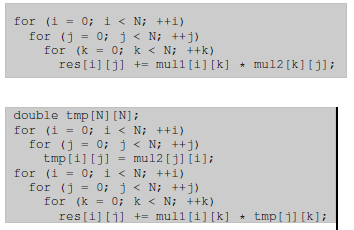
\includegraphics[scale=0.7]{matrix.png}
\\
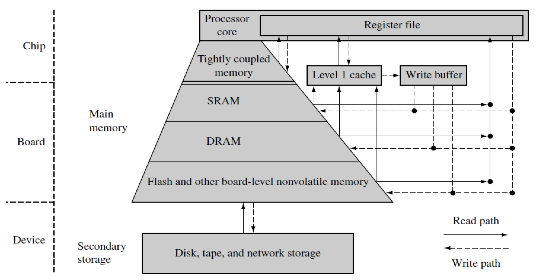
\includegraphics[scale=0.7]{cache.png}
\\
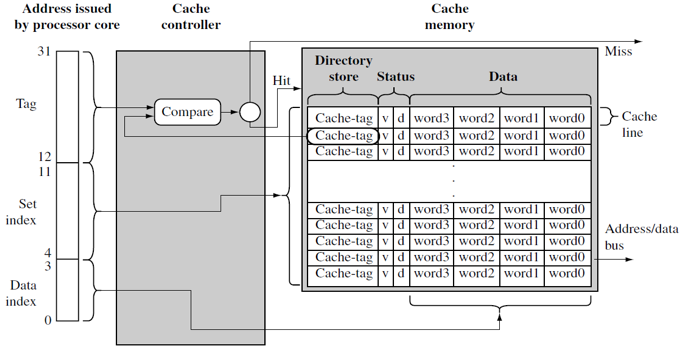
\includegraphics[scale=0.7]{cachecontroller.png}
\end{document}
